% !TeX root = ../main.tex
% Add the above to each chapter to make compiling the PDF easier in some editors.

\chapter{Appendix}\label{chapter:appendix}

\section{Network Architectures}

\subsection{Flux Network}
Input to the network is a grayscale image and output is 3 channel vector field.
The backbone of the network is based on Unet \cite{ronneberger2015}. The encoder and decoder of the Unet has four stages, and a center bottleneck layer, with $8, 16, 24, 32, 40$ filters respectively. The network has a theoretical field of view of $32\times378\times378$. Further details can be seen in \autoref{fig:network_blocks} and \autoref{fig:flux_net}.

\begin{figure}[ht]
	\centering
	
\includegraphics[width=\textwidth]{figures/network/legend.png}
	\caption{Network blocks used in Flux Network and Tracking Network.}
	\label{fig:network_blocks}
\end{figure}

\begin{figure}[ht]
	\centering
	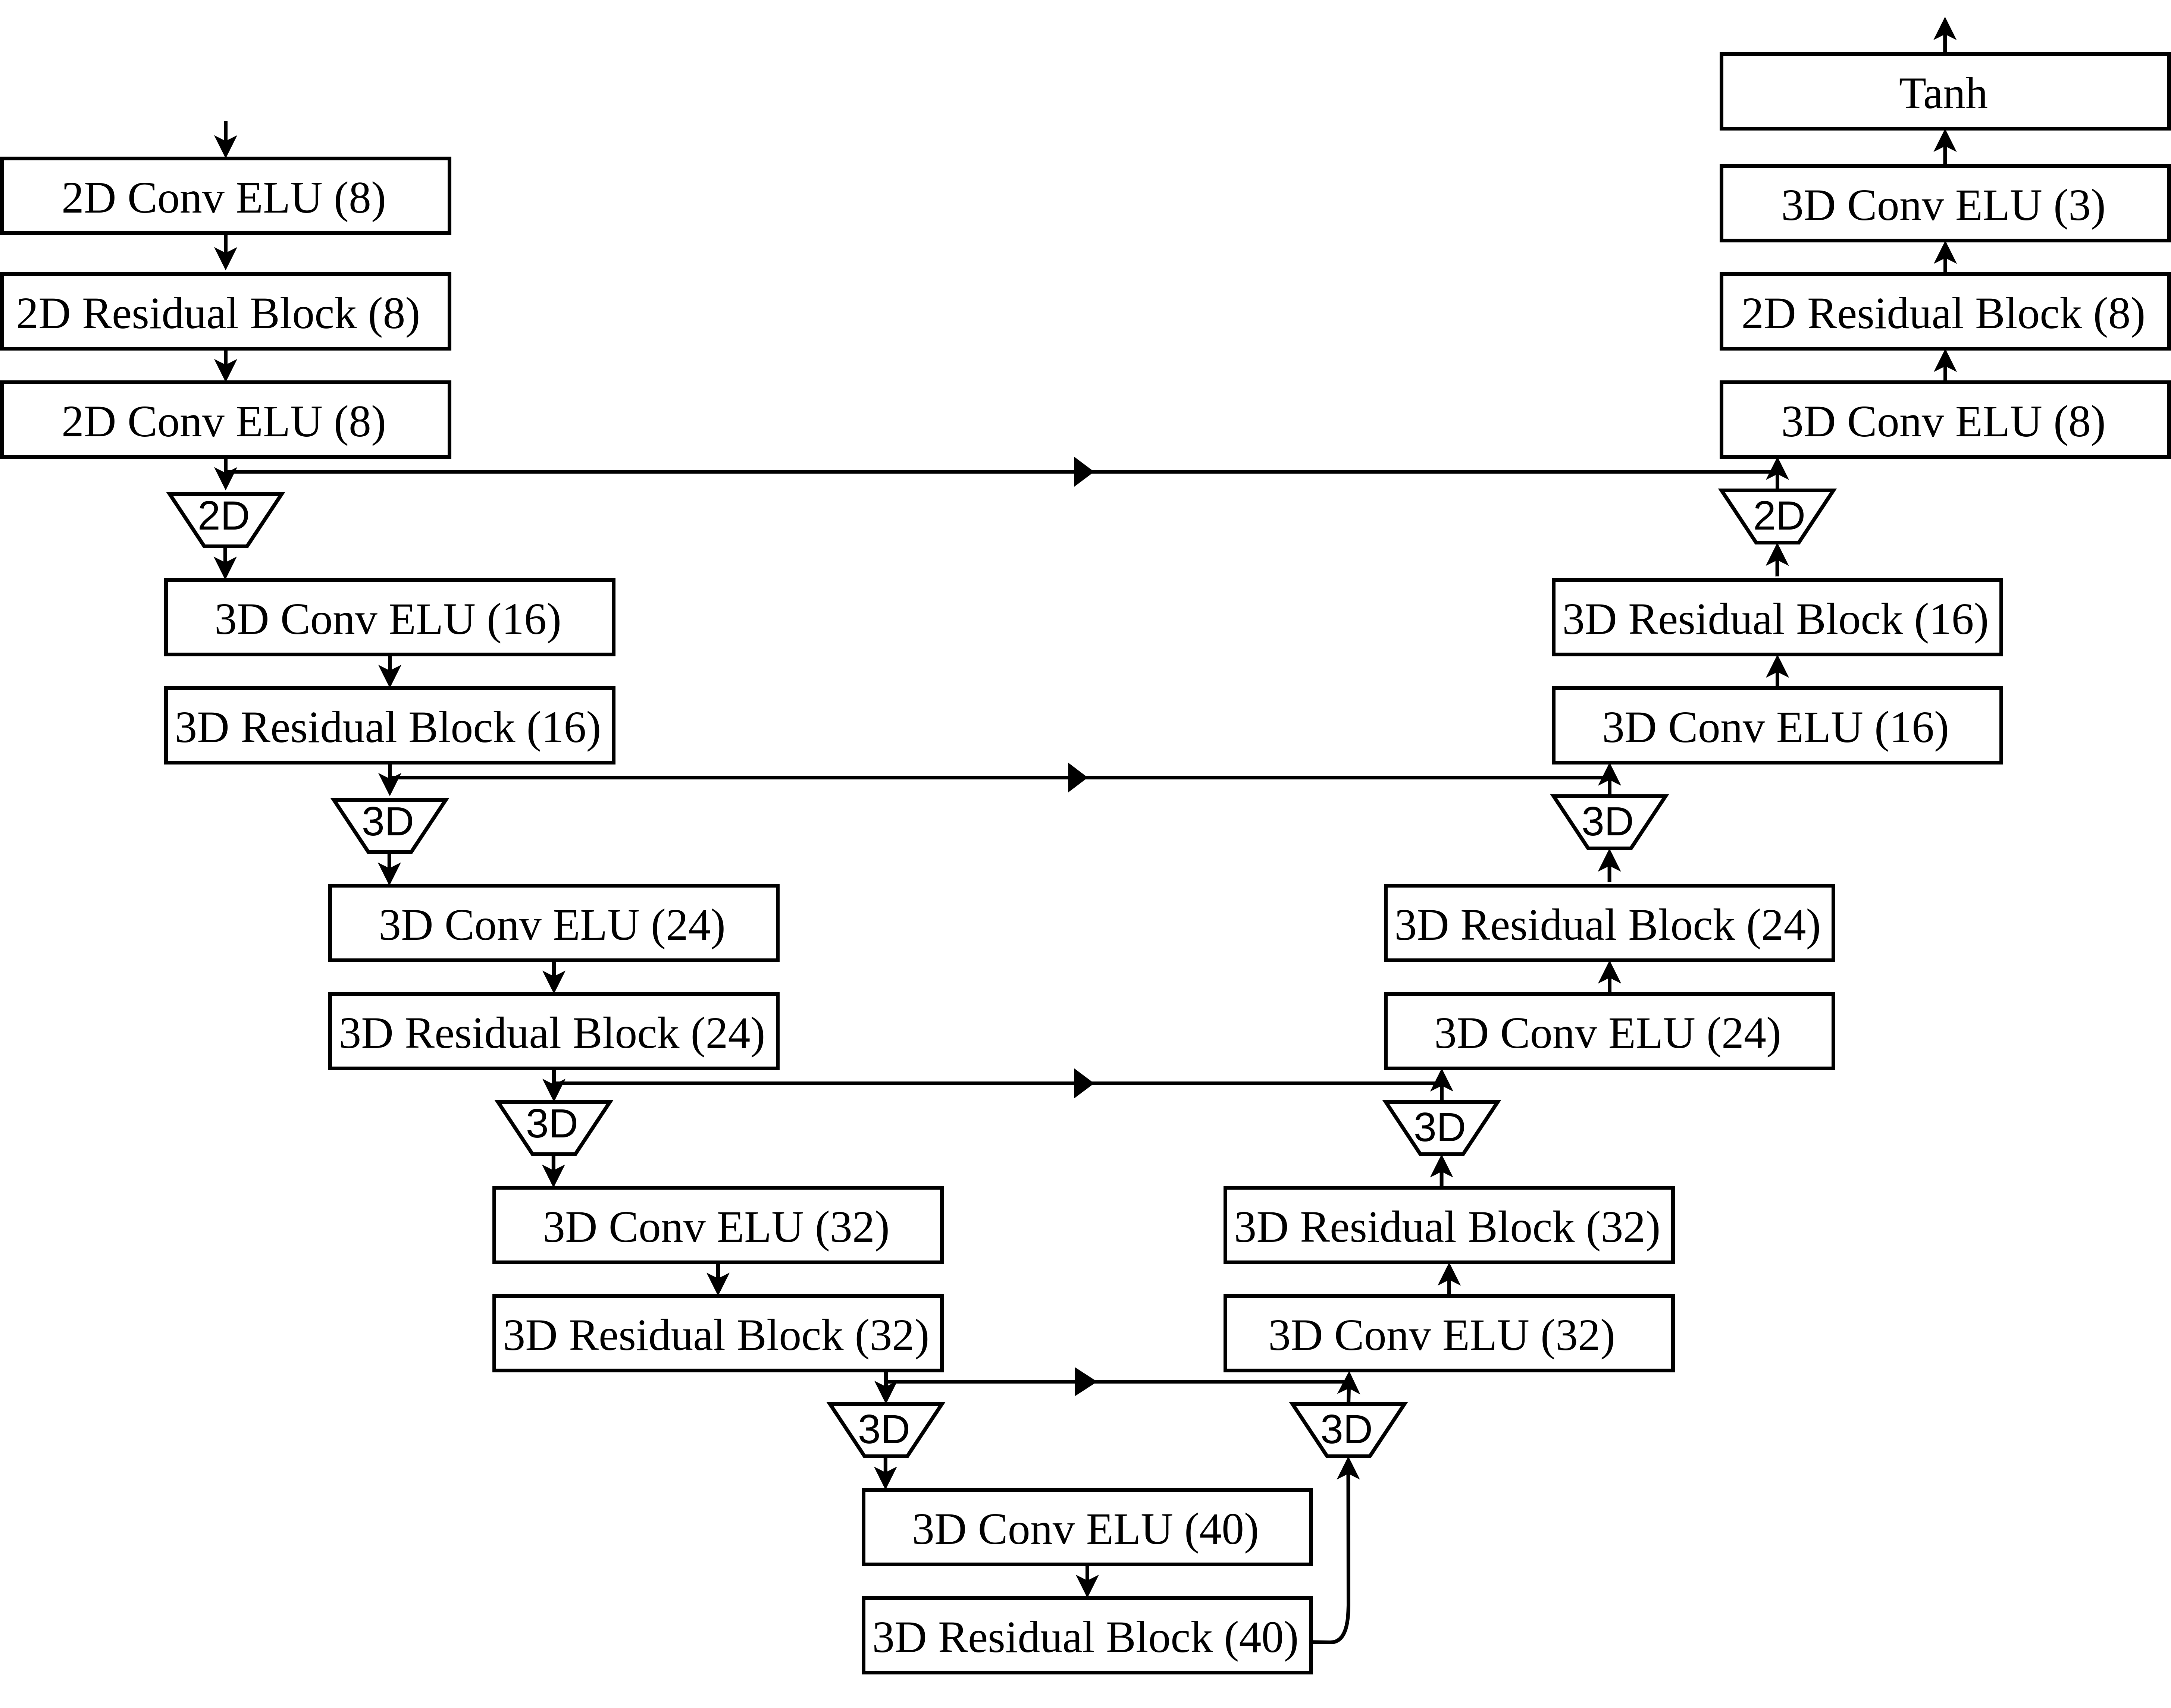
\includegraphics[width=\textwidth]{figures/network/flux_net.png}
	\caption{Flux Network. Input is a grayscale image of size $1\times64\times192\times192$. Output is the flux field of size $3\times64\times192\times192$.}
	\label{fig:flux_net}
\end{figure}


\subsection{Tracking Network}

Tracking Network is based on 3D convolution layers, a convolutional LSTM block and fully connected layers at the end. The details are show in \autoref{fig:direction_net}.

\begin{figure}[ht]
	\captionsetup[subfigure]{aboveskip=1pt,belowskip=1pt}
	\centering
	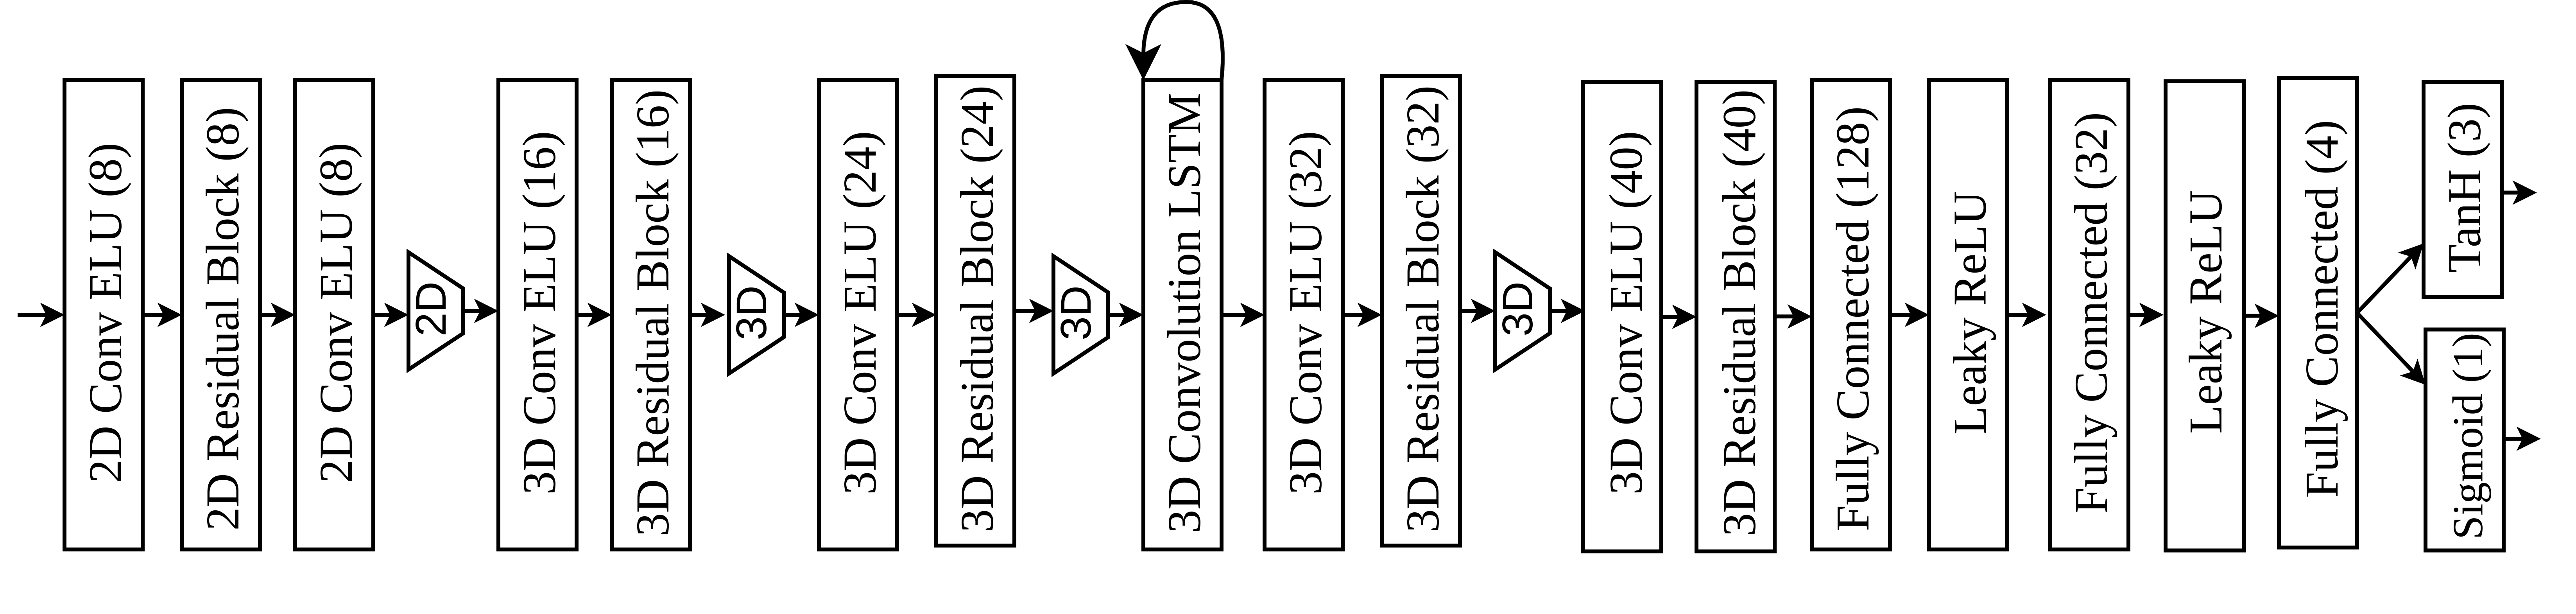
\includegraphics[width=\textwidth]{figures/network/direction_net.png}
	\caption{Tracking Network. Input is a $14\times16\times64\times64$ volume, comprising of input image, flux, start skeleton mask, other skeletons mask, and global features from Flux Network of channel sizes $1, 3, 1, 1, 8$ respectively. Outputs are 1) growing direction vector of size 3 and a scalar for the \it{\{continue-stop\}} probability.}
	\label{fig:direction_net}
	\vspace{-0.1in}
\end{figure}
